\chapter{Marco Teórico}

\section{Competencias de Drones Autónomos}

Las carreras de drones se han convertido en un deporte bastante popular en los últimos años. Resulta increíble pensar que, haciendo uso de única y exclusivamente una cámara de vuelo, los pilotos son capaces de abstraer la información necesaria del ambiente para ejecutar maniobras de vuelo con alta precisión y agilidad. 

A partir de lo anterior, la comunidad científica, en especial aquella dedicada al campo de la robótica, se ha visto bastante interesada en sustituir al piloto humano por meras unidades de cómputo y componentes electrónicos; es decir, hoy en día existe la tendencia a automatizar el vuelo de estos vehículos aéreos no tripulados,  de tal manera que, a partir de computadoras de placa única, sensores y algoritmos sofisticados de visión artificial, odometría y gestión y control de trayectoria de vuelo, se pueda obtener el mismo desempeño de vuelo que el otorgado por un piloto humano, e incluso, en algún punto, superarlo de manera significativa.

Sumando a lo ya expresado, se han creado una serie de instituciones y eventos con el fin de financiar, potenciar y motivar el desarrollo tecnológico en este campo emergente, dando lugar a lo que se conoce como \textit{carreras de drones autónomos}. Dentro de los eventos o competencias más significativas se encuentra el \textit{Autonomous Drone Racing (ADR)}\cite{moon2017iros}, llevado a cabo cada año en la Conferencia Internacional de Sistemas y Robots Inteligentes (IROS, por sus siglas en inglés),  el \textit{AlphaPilot Challenge (APC)}\cite{foehn2020alphapilot}, organizado por Lockheed Martin en colaboración con Nvidia y la Liga de Carrera de Drones (DRL); y \textit{Game of Drones (GOD)}\cite{madaan2020airsim}, gestionada por Microsoft para la Conferencia Anual de Sistemas de Procesamiento de Información Neuronal (NeurIPS) de 2019.

Los eventos anteriores representan un punto de encuentro a nivel internacional que ha permitido dirigir los esfuerzo e intelectos alrededor del mundo, a la propuesta de soluciones, ya sea de forma parcial o general, para el dilema ya expresado; y de hecho, es ahí en donde se ha presentado el estado del arte de este enfoque, pues se busca poner a prueba las implementaciones propuestas por los participantes en circuitos y retos con distintas características y composición. En las siguientes subsecciones se describe con más detalle las características, requisitos y relevancia de cada una de las competencias mencionadas.

\subsection{Autonomous Drone Racing}
A grandes rasgos, el ADR es una competencia que busca promover soluciones para vuelos autónomos ágiles en ambientes angostos de interiores. En el desafío se combinan técnicas y enfoques que buscan optimizar distintos parámetros de desempeño, como la generación de trayectoria de vuelo, el tiempo de recorrido de los circuitos, esquemas de control, detección de obstáculos, localización y mapeo, entre otros. 

El ADR debutó como evento en la edición de 2016 del IROS, en Daejeon, Corea. A partir de entonces siguió teniendo presencia en 3 ediciones más del IROS; en 2017 con sede en Vancouver, Canadá, en 2018 en Madrid, España y en 2019 Macao, China. Cabe recalcar que el IROS per se sigue llevando a cabo, sin embargo, la última ADR tuvo lugar en la edición 2019 de este evento, posiblemente por las restricciones derivadas en 2020 por la pandemia provocada por el virus SARS-CoV-2; además, la edición 2021 del IROS, se llevó a cabo de forma virtual.  

En general, en cada edición se propuso una única pista, dentro de una zona techada, con 5 pruebas de vuelo para los equipos participantes; velocidad de vuelo en línea recta a través de una serie de compuertas incompleta, vuelo en curva cerrada, recorrido de un circuito en zigzag, recorrido de un circuito en espiral y a través de compuertas cerradas y vuelo por un corredor con obstáculos dinámicos. 

En la edición de 2016, las compuertas fueron identificadas con un número embebido en un código QR, para facilitar su localización. El tamaño de los drones se limitó a un volumen máximo de  1 m x 1 m x 1 m; a los equipos se les compartieron detalles estructurales sobre el circuito antes de la competencia, por lo que les era posible generar mapas les pudieran auxiliar en la navegación del dron. Además, se les permitió el uso de cualquier tipo de sensor, siempre y cuando este estuviera montado en el chasis del vehículo; se utilizaron distintos tipos de sensores para su participación, incluyendo lidares, láseres, radares y sensores ultrasónicos.

En cada edición del ADR, las compuertas utilizadas para delimitar el circuito han conservado un característico color naranja; en cada evento los circuitos cumplieron con los requerimientos y pruebas mencionadas anterior mente, excepto en la edición 2019 en donde el circuito estuvo compuesto por dos grupos de compuertas LED, alfombras con patrones y luces controladas; además, el tamaño de este circuito fue reducido para producir una pista mucho más angosta, con el objetivo de incrementar la dificultad en el desafió \cite{rojas2021board}.   

Para cada equipo, la competencia comenzaba con el despegue del dron de forma manual, este era posicionado en un punto de inicio y en cuanto se diera la señal, los equipos cedían el control del dron a su sistema de piloto automático; es decir, se tenía que suspenderse toda clase de interacción humana con el sistema de vuelo del dron, y permitir que navegara de forma autónoma hasta completar el circuito. 



\subsection{AlphaPilot Challenge}
Como se mencionó, el APC es otra competencia enfocada en las carreras de drones autónomos, fue presentado como un reto de innovación con un gran premio de \$1 millón de dólares para el equipo ganador; la iniciativa fue creada y lanzada al público por Lockheed Martin en conjunto con La Liga de Carrera de drones, en 2019. El objetivo del desafío fue desarrollar un dron completamente autónomo que pudiera navegar por un circuito de vuelo utilizando visión por computadora; a diferencia de otras competencias, el APC no solo buscaba poner a prueba la capacidad de navegación de los sistemas, sino que, se buscaba explotar por completo los sistemas de vuelo, de tal forma que se buscó evaluar también la velocidad de vuelo y agilidad de las maniobras en una pista  más grande y compleja en comparación con la de ADR. 

Entonces, en el APC se buscó implementar soluciones más complejas que permitieran percibir el ambiente del dron por medio sistemas de visión artificial y que los sistemas de control de vuelo fueran capaces de llevar al límite la velocidad de navegación de este; el objetivo era claro, se buscaba ampliar el estado del arte y desarrollar implementaciones que pudieran competir con el desempeño de los mejores pilotos humanos. 

Más de 400 equipos participaron en la etapa de selección de esta primera edición del APC, y solamente los mejores 9 equipos clasificaron para poder participar en la competencia. La segunda fase del reto consistió en 3 carreras de clasificación, de donde se seleccionaron a 6 equipos finalistas. La etapa final de la competencia se disputó con un único circuito, donde los equipos compitieron por llevarse el gran premio de \$1 millón de dólares. Los ganadores de cada etapa y carrera de selección fueron filtrados a partir del tiempo que les tomó completar los circuitos; cada participante contó con 3 intentos para completar los circuitos tan rápido como les fuese posible y sin ningún otro competidor o adversario en la pista.

En cada carrera, los drones empezaban en un podio desde donde tenían que despegar y navegar por una secuencia de compuertas con formar distintas y en un orden predefinido. A diferencia del ADR, a los equipos del APC solo se les informó de la estructura de la pista momentos antes de competir; es decir, no podían hacer uso de un mapa detallado para definir la trayectoria de vuelo que tenía que seguir su dron, sino que, tenía que implementar soluciones que se pudieran adaptar en tiempo real a la posición de las compuertas. Se había estimado una longitud de aproximadamente 300 m para cada pista, sin embargo, debido a dificultades técnicas, la pista de mayor longitud fue la de la carrera final, con una longitud aproximada de 74 m\cite{foehn2020alphapilot}.   

Por último, las características del dron utilizado fueron estandarizadas, por lo que a cada equipo se les otorgó el mismo modelo de dron. Además, a todos los equipos se les facilitó una computadora de vuelo \textit{NVIDIA Jetson Xavier}, para la interfaz con los sensores y actuadores de navegación y también fungió como la unidad de procesamiento para llevar a cabo el vuelo autónomo. El arreglo de sensores a bordo de dron se conformó por un par de cámaras estero con  vista frontal a $30^\circ$, una unidad de medición inercial (IMU), un telémetro láser (LRF); la tabla 1 muestra las especificaciones técnicas de los sensores utilizados. Por último, los drones también estaban equipados con un controlador de vuelo encargado de controlar el empuje y la velocidad angular.

\begin{table}
    \centering
    \begin{tabular}{llll}
        \hline
        Sensor & Modelo & Frecuencia & Detalles\\
        \hline
        Cámara & Leopard Imaging IMX 264 & $60 Hz$ & resolución de 1200 x 720\\
        IMU & Bosch BM1088 & $430 Hz$ & rango: $\pm 24 \text{ g}$, $\pm 34.5 \text{rad/s}$\\
         & & & resolución: $7e^{-4}\text{g, } 1e^{-3}\text{rads/s}$\\
        LRF & Garmin LIDAR-Lite v3 & $120 Hz$ & rango: $1-40$ m\\
        & & & resolución: $0.01 \text{ m}$\\
        \hline
    \end{tabular}
    \caption{Especificaciones de sensores utilizados en el APC \cite{foehn2020alphapilot}}
    \label{tab:sensors}
\end{table}

\subsection{Game of Drones}
En la tercera edición de la Conferencia Anual de Sistemas de Procesamiento de Información Neuronal (NeurIPS), en 2019, el equipo de desarrollo de AirSim\cite{foehn2020alphapilot} en conjunto con la Universidad de Stanford y la Universidad de Zúrich buscaron fomentar el avance de las tecnologías utilizadas den las carreras de drones, gestionando la competencia Game of Drones.

De manera similar a las competencias anteriores, el GOD buscó explotar el potencial de los algoritmos de machine learning y visión por computadora, junto con los avances en cuestión de técnicas de planificación de trayectoria, control y estimación de estado de quadrotores; sin embargo, a diferencia de los otros eventos, el GOD se basó completamente en la utilización de un simulador de vuelo con gráficas foto-realistas para la implementación de las propuestas desarrolladas por los equipos. 

El simulador utilizado para la competencia  fue Microsoft AirSim\cite{airsim2017fsr}, el cual fue desarrollado con el objetivo de hacer más accesible el ámbito de las carreras de drones para ingenieros e investigadores, que tiene un conocimiento bastante amplio sobre algoritmos de machine learning e inteligencia artificial, pero que quizás no estén tan familiarizados con el hardware utilizado por estos sistemas de robótica. AirSim se define como un ambiente de simulación para multi-rotores, que integra un motor de físicas de consumo reducido, controlador de vuelo, sensores inerciales, y gracias al uso del motor gráfico Unreal Engine (UE), cuenta con un ambiente con gráficos foto-realistas. Además, también ofrece una API (Application Programming Interface) que permite interactuar y comunicarse con los algoritmos de machine learning, y también provee datos sobre el progreso del recorrido, el desempeño del dron y la habilidad de imponer reglas o normas para la carrera, asociadas a infracciones por colisiones y descalificaciones dentro de la competencia.

La competencia se enfocó en control y planificación de trayectoria, visión artificial y evasión de obstáculos (otro dron oponente). Lo anterior se llevó a cabo en tres niveles con base en el enfoque: 

\textbf{Nivel 1} - Planificación de trayectoria: cada circuito estuvo limitado a dos drones a la vez, en donde uno era el perteneciente al equipo participante y el otro era un dron oponente implementado por el staff de Microsoft. El objetivo fue atravesar todas las compuertas en el menor tiempo posible, evitando colisionar con el dron oponente. La posición de las compuertas y de ambos drones fue proveída a través de la API del simulador. El dron oponente contaba con un algoritmo de trayectoria óptima y volaba con una serie de waypoints generados al azar para cruzar por la sección transversal de cada compuerta.

\textbf{Nivel 2} - Percepción: en esta modalidad, la posición de las compuertas contenía ruido, no había dron oponente y la siguiente compuerta a cruzar no siempre se encontraba a la vista; la posición proveída por la API ayudaría a dirigir al dron en la dirección correcta, sin embargo, el vehículo tenía que valerse de su algoritmo de visión artificial para completar el circuito de manera satisfactoria.

\textbf{Nivel 3} - Percepción y planificación de trayectoria: esta modalidad resulto de la combinación de los dos niveles anteriores. A los participantes se les preveía con datos sobre la posición de las compuertas y había un dron adversario; el objetivo era completar el circuito evitando cualquier colisión con el adversario.

Por último, la competencia consistió de dos etapas, una de clasificación y una ronda para los finalistas. Se registraron 117 participantes, pero solamente 16 calificaron para la competencia.


 
\section{Robot Operating System (ROS)}

\subsection{Concepto}

De acuerdo con su sitio oficial\cite{rosFoxy}, ROS (del inglés, Robot Operating System) es un conjunto de herramientas y librerías de software para robótica desarrolladas por Open Robotics\cite{openRobotics} bajo el paradigma de software libre u open-source. Este entorno de trabajo destaca por contener algoritmos de última generación y herramientas de desarrollo avanzadas,  que permiten la creación, implementación y reutilización de código para todo tipo de proyectos de robótica.

ROS 1, la primera versión del entorno de trabajo, surgió en 2007 como un ambiente de desarrollo para el PR2 robot, un robot de servicio diseñado para trabajar con personas y creado por la empresa The Willow Garage. Sin embargo, los creadores de ROS buscaban que el entorno de trabajo no se viera limitado a un solo modelo de robot, sino que, pudiera ofrecer herramientas de software para más tipos y modelos de robots, por lo que ROS adquirió varias capas de abstracción mediante la implementación de interfaces para el manejo de mensajes, lo que dio lugar a que el software desarrollado mediante ROS pudiera ser reutilizado en más robots.   

Algunas características que destacan en esta etapa temprana de ROS son:
\begin{itemize}
    \item Gestión de un solo robot
    \item Sin requerimientos de aplicación en tiempo real
    \item Excelente conectividad a la red
    \item Usado principalmente en el ámbito académico y de investigación
\end{itemize}

Hoy en día, ROS es utilizado en una amplia gama de robots, desde robots con ruedas y con forma humanoide, hasta brazos industriales, vehículos aéreos y mucho más. Sin embargo, ha pasado bastante tiempo desde el lanzamiento de la primera versión de ROS, y las necesidades y estándares de la industria han cambiado al igual que el paradigma y la filosofía detrás del desarrollo de ROS. Dicho lo anterior, es evidente que ROS ha adquirido una alta relevancia desde su creación; sin embargo, existen muchas limitaciones asociadas a la manera en que ROS fue diseñado. 

\subsection{Conceptos básicos de ROS}

\textbf{Paquetes:} son la unidad principal para organizar software en ROS. Un paquete puede contener procesos (nodos), liberarías, conjuntos de datos, archivos de configuración o cualquier otro tipo de archivo que pertenezca a un conjunto funcional.  Los paquetes representan la unidad atómica en ROS.

\textbf{Tipos de mensajes:} descripción de mensajes, definen la estructura de los datos para los mensajes manejados por ROS.

\textbf{Tipos de servicios:} descripción de servicios, define la estructura solicitada o enviada para los datos utilizados en los servicios de ROS.

\textbf{Nodos:} son procesos que llevan a cabo cálculos. ROS está diseñado para ser modular. Un sistema robótico generalmente está compuesto por múltiples nodos encargos de distintas tareas como la lectura de un sensor, control de un actuador, ejecución de algoritmos, etc.

\textbf{Mensajes:} forma de comunicación entre nodos. Son estructuras de datos para el intercambio de información entre nodos.

\textbf{Topics:} canales de transporte por donde se envían los mensajes, a través de una dinámica de editor y subscriptor. Un nodo envía un mensaje publicándolo en un topic; el topic es el nombre utilizado para identificar el contenido del mensaje.

\textbf{Servicios:} tienen una función similar a los topics, sin embargo, los servicios generan una respuesta/interacción a partir de las solicitudes enviadas.

\textbf{Bags:} registros en donde se almacenan los datos de un mensaje enviado.

\subsection{Las limitaciones de ROS 1}

La forma en que se manejan las comunicaciones entre nodos de cómputos distribuidos en ROS 1 dificulta la integración entre dispositivos de hardware (sensores, actuadores, etc.). Para realizar una red de procesamiento distribuido en ROS 1, es necesario contar con un dispositivo maestro que inicia antes de cualquier otro nodo. Además, las comunicaciones entre nodos se llevan a cabo utilizando el protocolo de llamada XML-RPC, el cual pose una dependencia significativa cuando se implementa en cualquier sistema de recursos limitados o microcontroladores, debido a su naturaleza recursiva. En vez de lo anterior, es muy común que se utilice un controlador con un protocolo de comunicaciones propio para realizar la interacción entre los dispositivos.

En ROS 1, los nodos comúnmente utilizan la API \textit{Node}, la cual implementa su propia función \text{main}, en vez de la API \textit{Nodelet} para compilar librerías compartidas. Debido a lo anterior, el desarrollador tiene que escoger entre una de estas dos APIs, y el proceso para convertir de una API a otra no es trivial y requiere una inversión de tiempo considerable.

En cuanto al proceso de lanzamiento, el sistema de lanzamiento de ROS 1 solo inicializa un conjunto de procesos, y no provee ningún tipo de retroalimentación fuera de sí el proceso fue iniciado o no. Sin embargo, es común que los desarrolladores escriban sus procesos para que esperen una cierta cantidad de tiempo o una bandera de estado, que indique que todo está bien antes de comenzar a procesar los datos. 

Además, en sistemas complejos la observabilidad de los procesos y la posibilidad de una configuración dinámica se vuelven mucho más relevantes. En ROS 1 los nodos no tiene ningún estado asociado y solo algunos componentes una interfaz para obtener información o manipular el sistema durante su ejecución.  
   
A partir de lo anterior, en 2014 una nueva versión de ROS con un enfoque y estructura distinta es anunciada por Open Robotics.  ROS 2 surge como un completo rediseño para lo que había sido el entorno de trabajo hasta entonces, con esta reestructuración se busca cubrir necesidades y funcionalidades que no habían sido consideradas con  ROS 1, pero que habían sido exigidas por la comunidad y la industria. Lo anterior dio lugar al desarrollo de un nuevo conjunto de paquetes con cambios en API general, arquitectura y comunicación. 

\subsection{¿Por qué ROS 2?}

Como se mencionó anteriormente, ROS surgió con la idea de satisfacer las necesidades de un único modelo de robot, y lo logró; Por otro lado, a pesar de haber ampliado el framework para funcionar para otros dispositivos, como ya se mencionó, con el paso del tiempo los desarrolladores del proyecto de algunas características importantes de las que carece ROS 1, pues si bien es cierto que en lo últimos años ROS ha adquirido una importante relevancia, su uso se ha visto limitado a aplicaciones con fines académicos y no ha podido despegar en el sector industrial debido a las limitaciones con las que cuenta, dentro de ellas cabe mencionar el hecho de no estar diseñado para trabajar con sistemas en tiempo real, además de carecer de estándares de seguridad para llevar a cabo certificaciones de este tipo. 

Las características mencionadas anteriormente no son para nada triviales y modificar el framework de ROS 1 para implementarlas implica realizar una gran cantidad de cambios, los cuales pueden provocar inestabilidad en el proyecto, pues son adiciones que no se planificaron dentro de la etapa de diseño del framework. Entonces, la opción más razonable para el quipo de desarrollo fue crear un nuevo framework desde cero; ROS 2. 

Dicho lo anterior, se tiene definidos nuevos casos de uso que dirigen el desarrollo de ROS 2, al mencionar algunos de los más importantes se encuentran los siguientes:

\begin{itemize}
    \item Sistemas compuestos por múltiples robots: existe la posibilidad de implementarlos en ROS 1, pero no existe un estándar o un acercamiento unificado que permita el desarrollo para este tipo de sistemas.
    \item Sistemas embebidos: se tiene por objetivo que la implementación de ROS en sistemas embebidos, como computadoras de placa única y microcontroladores, no sea a través de un controlador de dispositivo, sino que, sea posibilidad configurar el dispositivo como una computadora normal.
    \item Sistemas en tiempo real: soporte para este tipo de sistemas de forma nativa en ROS, ofreciendo comunicación inter-proceso e inter-máquina.
    \item Redes no ideales: desempeño estandarizado incluso si la conectividad de red es deficiente.
    \item Ambientes de producción: seguir enfocando el desarrollo al área de investigación, pero facilitar la evolución de un mero prototipo a una aplicación comercial.
    \item Patrones para el desarrollo y estructura de sistemas: conservar la flexibilidad en el desarrollo de soluciones pero proveer estándares y herramientas de desarrollo enfocadas al manejo de un ciclo de vida y configuraciones estáticas para su lanzamiento.
\end{itemize}

ROS 2 propone una arquitectura en donde es posible implementar el protocolo de comunicación entre nodos directamente en cualquier sistema embebido, de tal forma que cualquier dispositivo ROS dentro de la red sea descubierto de forma automática por la interfaz de ROS; se implementa una comunicación más descentralizada pues ya no existe la figura de maestro y se implementa una lógica de intercambio de información del tipo DDS (Data Distribution Service), la cual está pensada para sistemas en tiempo real. Además, la forma de crear nodos en ROS 2 está pensada para que el usuario sea capaz de decidir el tiempo  y la forma de lanzamiento de un nodo; cada nodo puede ser lanzado en procesos distintos para facilitar la depuración de estos, o, pueden ser integrados a un solo proceso para obtener un mejor rendimiento y aprovechar la comunicación inter-proceso.  

Lo anterior también conlleva un cambio significativo dentro de la API de ROS; se rediseñó con el fin de mejorarla, de tal forma que los conceptos clave de la versión anterior se conservaron, pero se ofrece una gran mejora y experiencia al usarla. Esto significa que la API de ROS 1 no es compatible con la de ROS 2, y viceversa; sin embargo, se busca que el código de ambas versiones pueda coexistir en un mismo sistema e incluso que cuenten con cierto tipo de interacción; esto permite que la transición entre ambas versiones sea de forma gradual y práctica.

La tabla \ref{tab:rosd} presenta un resumen de las distribuciones de ROS 2 desarrolladas hasta el momento, en ella se indica la fecha de lanzamiento de cada una y el periodo en el que se dejara de ofrecer soporte para estas. Cabe destacar que cada distribución de ROS esta asociada a una única versión LTS (Long Term Support) de Ubuntu.

En cuanto a ROS 1, actualmente se encuentra activas dos distribuciones, Melodic Morenia y Noetic Ninjemys. Siendo esta última la versión final de ROS 1, cuyo objetivo es implementar Python 3 para aquellas organizaciones y empresas que necesitan seguir trabajando con ROS 1 por un tiempo. Por otro lado, el servicio de soporte técnico para esta última versión terminará en mayo de 2025, de tal forma que se tiene hasta entonces para que los usuarios de ROS 1 migren a ROS 2, si es que desean seguir utilizando un framework con un desarrollo activo por parte de Open Robotics.

\begin{table}
    \centering
    \begin{tabular}{lll}
        \hline
        \textbf{Distribución} & \textbf{Fecha de lanzamiento} & \textbf{Fin de vida útil}\\
        \hline \hline
        Humble Hawksbill & Mayo 23, 2022 & No especificada\\
        Galactic Geochelone & Mayo 23, 2021 & Noviembre 2022\\
        Foxy Fitzroy & Junio 5, 2020 & Mayo 2023\\
        Eloquent Elusor & Noviembre  22, 2019 & Noviembre 2020\\
        Dashing Diademata & Mayo 31, 2019 & Mayo 2021\\
        Crystal Clemmys & Diciembre 14, 2018 & Diciembre 2019\\
        Bouncy Bolson & Julio 2, 2018 & Julio 2019\\
        Ardent Apalone & Diciembre 8, 2017 & Diciembre 2018\\
        beta3 & Septiembre 13, 2017 & Diciembre 2017\\
        beta2 & Julio 5, 2017 & Septiembre 2017\\
        beta1 & Diciembre 19, 2016 & Julio 2017\\
        alpha1 - alpha8 & Agosto 13, 2015 & Diciembre 2016\\
        \hline \hline
    \end{tabular}
    \caption{Lista de distribuciones de ROS 2}
    \label{tab:rosd}
\end{table}

\subsection{Diferencias entre ROS 1 y ROS 2}
Con base en todo lo que se mencionó en las secciones anteriores, la tabla \ref{tab:ROS1ROS2} hace un compilado de todas las diferencias importantes entre ROS 1 y ROS 2.

\begin{table}[ht]
    \centering
    \begin{tabular}{p{0.2\linewidth} p{0.35\linewidth}p{0.35\linewidth}}
        \hline
        \textbf{Característica} & \textbf{ROS 1} & \textbf{ROS 2} \\ \hline \hline
        Plataformas & Únicamente soporta de forma nativa Ubuntu. & Soporta Ubuntu, Mac OS X y Windows 10. \\ \hline
        Programación & Trabaja con C++03 y Python 2; Python 3 en su última versión con plan de soporte. & Utiliza C++11 de forma extensiva y usa algunas partes de C++14 y Python a partir de la versión 3.5.\\ \hline
        Comunicación & Utiliza una capa de comunicación diseñada desde cero (XML-RPC) & Adopta un protocolo ya definido (DDS) \\ \hline
        Compilación & Utiliza \textit{catkin} para compilar e instalar sus paquetes & Implementa \textit{Ament}, un nuevo sistema de compilación que integra a \textit{colcon}.\\ \hline
        POO & No hay un estándares, cada implementación es única & Existen pautas definidas par escribir los nodos \\ \hline
        Archivos de lanzamiento & Se crean utilizando XML y Python, sin embargo, de este último no hay documentación sobre como hacerlo & Permite crearlos de forma nativa en Python ofreciendo una mayor personalización en cada archivo. \\ \hline
        Servicios & Son síncronos & Son asíncronos. \\ \hline
        Paquetes & Se crean los paquetes y se añaden archivos de forma indistinta & Se tiene que especificar si el paquete se basara en Python o C++.\\ \hline \hline
    \end{tabular}
    \caption{ROS 1 vs. ROS 2}
    \label{tab:ROS1ROS2}
\end{table}

Tomando como referencia la tabla \ref{tab:ROS1ROS2} es evidente que el paradigma que rige el diseño de ROS 2 es por mucho muy superior en cuanto a estructura, practicidad y mantenibilidad; sin embargo, hoy en día muchas de las implementaciones que estas relacionadas con ROS son realizadas con la primera versión del framework, por lo que ROS 1 sigue teniendo una presencia bastante sólida en comparación con la nueva versión desarrollada. Esto tenderá a cambiar con el paso del tiempo, pero se trata de un proceso gradual que puede llegar a tomar años.

Por otro lado, la comunidad de ROS recomienda a los usuarios nuevos formar parte de la transición e iniciar por aprender los fundamentos de ROS 2. En contraste con lo anterior, aprender las implicaciones y la forma de trabajo de ROS 1 puede resultar benéfico para los nuevos usuarios también, pues otorgaría una formación más sólida con el objetivo de tener un panorama más detallado sobre la forma de trabajo con ROS, en general.

Por último, existe otro obstáculo que dificulta la transición hacía la nueva versión de ROS, y es que para el usuario promedio puede que el porteo de proyecto de una versión a otra no conlleve tanto esfuerzo, en especial si se trata de proyectos pequeños; sin embargo, al hablar de organizaciones y empresas con proyectos a gran escala, esta actividad puede llegar a representar una cantidad considerable de tiempo y esfuerzo, por lo que es entendible que en estos casos se opte por seguir utilizando ROS 1, y que para nuevos proyectos se opte por utilizar ROS 2.

\section{Visión Artificial}

\subsection{Concepto}

La visión artificial o visión por computadora es un campo de la informática que tiene por objetivo extraer información de imágenes, y a pesar de que el concepto suene sencillo, ha representado un reto a lo largo del tiempo. Se le ha dedicado una gran cantidad de esfuerzo por parte de las mentes más brillantes y creativas de las últimas décadas, y a pesar de ello, el avance tecnológico parece indicar que aún no se logra por completo el objetivo de desarrollar una máquina de propósito general capaz de observar la realidad como lo hace el sistema conjunto del ojo y el cerebro humano.



\subsection{Segmentación de color utilizando el modelo HSV}

Generalmente, las imágenes digitales se encuentran definidas bajo un modelo de color de tres componentes: rojo, verde y azul (RGB), en donde a cada color se le asigna una matriz de las mismas dimensiones de la imagen, a tal forma que las tres matrices en conjunto conforman la concentración de color en los píxeles de la imagen en cuestión \cite{saravanakumar2011multiple}.

La concentración de cada color está definida por 8 bits; es decir, este parámetro puede tener un valor entre el 0 y el 255, que representan la menor y mayor concentración, respectivamente. El modelo de color RGB representa una forma sencilla para representar la concentración de color en una imagen, sin embargo, cuando se requiere buscar una tonalidad de color especifica en una imagen, utilizando este espacio de color, la situación puede llegar a complicarse cuando existen cambios de iluminación en el ambiente. 

Debido a lo anterior, cuando se quiere realizar operaciones de procesamiento de imágenes, se suele cambiar el modelo de color de la imagen de RBG a HSV, pues este espacio de color permite manejar los cambios de iluminación con más facilidad y utiliza un sistema para la definición del tono mucho más sencillo de utilizar. 

De manera similar e intuitiva, el espacio de color HSV está compuesto por tres parámetros para la definición de la concentración de color: el matiz (hue; H), la saturación (saturation; S) y el valor (value; V). Estos tres parámetros son organizados en una lista en el orden mencionado, y contienen un rango de valor asociado a cada uno. A continuación, la tabla \ref{tab:hsv_param} contiene la descripción de los parámetros utilizados por este modelo de color así como su rango de valores.

\begin{table}[ht]
    \centering
    \begin{tabular}{lll}
        \hline
        Parámetro & Descripción & Rango\\
        \hline \hline
        Matiz & La tonalidad del color & 0 - 179\\
        Saturación & La tonalidad grisácea del color & 0 - 255\\
        Valor & brillo del color & 0 - 255\\
        \hline \hline
    \end{tabular}
    \caption{Parámetros del espacio de color HSV}
    \label{tab:hsv_param}
\end{table}

\subsection{OpenCV}

\subsubsection{Concepto}

De acuerdo con su documentación oficial \cite{OpenCV}, OpenCV (del inglés, Open Source Computer Vision Library) es una librería multiplataforma de código abierto que fue diseñada para realizar procesamiento de imágenes en tiempo real, contiene una cantidad considerable de algoritmos de visión artificial, por lo que, es considerada un estándar para implementar aplicaciones en donde es necesario utilizar visión por computadora; está escrita en C/C++ y puede ser instalada en Linux, Windows y Mac OS X. Además, cuenta con interfaces para Python, Ruby, Matlab y otros lenguajes de programación. 

\subsubsection{Historia}
La primera versión alfa de OpenCV surgió a inicios de 1999, fue desarrollada por Intel con objetivos de investigación en aplicaciones de uso intensivo de CPU. En una visita al MIT, uno de los investigadores de Intel descubrió que un grupo de estudiantes habían desarrollado una infraestructura bastante sólida de visión por computadora, de tal forma que en vez de crear sus propias librerías desde cero, los estudiantes se compartían una serie de código fuente base, con el que podían llevar a cabo sus propias implementaciones, reduciendo el tiempo de desarrollo. 

De esta manera, OpenCV fue concebida como una infraestructura estándar que buscaba estar disponible para cualquier desarrollador alrededor del mundo. El desarrollo y optimización de la librería fue delegado a un grupo de expertos pertenecientes a Intel, en Rusia \cite{bradski2008learning}. Vadim Pisarevsky fue el líder del proyecto y participó de forma activa en la optimización y codificación de la librería, tal que gran parte del código desarrollado por él continúa siendo el núcleo funcional de la librería. En conjunto con Vadim, Victor Eruhimov apoyó en el desarrollo prematuro de la infraestructura, al igual que Valery Kuriakin, quien gestionó el laboratorio y aportó de forma continua al proyecto. 

A partir de lo anterior, OpenCV basó su desarrollo en algunos pilares u objetivos:

\begin{itemize}
    \item Proveer una infraestructura para visión artificial, no solo abierta, sino también optimizada; evitar reinventar la rueda.
    \item Descentralizar el conocimiento, poniendo al alcance de cualquier desarrollador una librería base que permitiera crear código con mejor legibilidad y más portabilidad.
    \item Potenciar aplicaciones comerciales de visión por computadora, ofreciendo código gratuito y de uso libre, con términos y condiciones de uso que no obligaran al desarrollador a publicar su aplicación como código libre.
\end{itemize}

En cualquier proyecto de código abierto, la participación de la comunidad es de suma importancia, pues el conjunto de esfuerzos es lo que permite que el proyecto se vuelva autosustentable; OpenCV no es la excepción, pues una cantidad considerable de usuarios han contribuido a su desarrollo, a tal grado que, se puede decir que ya no pertenece a Intel, sino a su propia comunidad. Se estima que la librería ha sido descargada más de dos millones de veces \cite{bradski2008learning}, creciendo de forma continua con un aproximado de hasta 26,000 descargar por mes. 

Hoy en día, OpenCV es utilizada en áreas como segmentación y reconocimiento, identificación de objetos, reconocimiento facial, seguimiento de movimiento, realidad aumentada, percepción de profundidad, calibración multi-cámara, entre muchas otras más \cite{garcia2015learning}. La explotación y el esfuerzo dedicado a la librería ha sido tal que, la infraestructura ya viene con módulos que integran de modelos estadísticos de machine learning.

\subsubsection{Características}
OpenCV fue diseñado con una estructura modular, es decir, el paquete en su conjunto está formado por una serie de librerías compartidas o estáticas. La tabla \ref{tab:OpenCV} presenta la lista de módulos incluidos en la paquetería, así como su respectiva descripcción.

\begin{table}[ht]
    \centering
    \begin{tabular}{p{0.3\linewidth}p{0.6\linewidth}}
        \hline
        \textbf{Módulo} & \textbf{Descripción}\\ \hline \hline
        Funcionalidad nuclear & Define las estructura de datos base e incluye funciones altamente sofisticadas para operaciones con arreglos multidimensionales y funciones utilizadas por otros módulos \\ \hline
        Procesamiento de imágenes & Incluye filtros lineales y no lineales para el procesamiento de imágenes, transformaciones geométricas, conversión de espacio de color, histogramas y más.\\ \hline
        Análisis de video & Constituido por funciones para estimación de movimiento, extracción de fondo, y algoritmos para seguimiento de objetos.\\ \hline
        Calibración de cámaras y reconstrucción 3D & Algoritmos multi-geométricos básicos, estimación de posición de objetos, reconstrucción  3D de elementos.\\ \hline
        Funcionalidades en 2D &  Detectores de características, descriptores y descriptores enlazadores\\ \hline
        Detección de objetos & Detección de objetos e instancias de clases especificadas.\\ \hline
        Interfaz gráfica de alto nivel & Interfaz fácil de utilizar con funcionalidades simples\\ \hline
        E/S de video & Interfaces para captura de video y codecs.\\ \hline 
        Otras & OpenCV cuenta con muchos más módulos, para más información consultar la documentación oficial \cite{OpenCV}\\ \hline \hline
    \end{tabular}
    \caption{Módulos de OpenCV}
    \label{tab:OpenCV}
\end{table}

\section{Software in The Loop}

El paradigma de simulación de Software in The Loop (SIL) conlleva la generación de un código fuente compilado a partir de un modelo matemático simulado, de tal forma que se crea un ambiente de simulación práctico para el desarrollo y validación de estrategias de control para sistemas complejos y de gran escala \cite{SIL_OPAL}. 

Con SIL, los ingenieros pueden utilizar una computadora de escritorio para interactuar con la simulación y modificar su código fuente, integrando su algoritmo de control a una planta virtual, substituyendo los prototipos costosos o los bancos de pruebas complejos. El SIL posibilita las pruebas del software antes de la inicialización de la fase de prototipaje, mejorando de forma significativa los tiempos del ciclo de desarrollo del sistema. 

Complementando lo anterior, la simulación de SIL permite detectar bugs o defectos en el código fuente en etapas tempranas de del ciclo de desarrollo, reduciendo los costos derivados de la solución de estos errores en etapas más avanzadas del desarrollo del sistema, cuando el número de componentes e interacciones entre ellos son más complejas y numerosas. 

A manera general, la simulación de SIL contempla la simulación del comportamiento de un algoritmo de control sobre el modelo de una planta o proceso; a diferencia otros paradigmas como Hardware in The Loop (HIL, \citet{HIL_OPAL})  o Rapid Control Prototyping (RCP, \citet{RCP_OPAL}), en una simulación de SIL tanto el sistema de control como el proceso de interés son completamente simulados a partir de modelos matemáticos; es decir, no se requiere ningún tipo de prototipaje físico más que el dispositivo simulador y una computadora para interactuar con la simulación.


Algunas de las ventajas inherentes del paradigma de SIL son: 

\begin{itemize}
    \item Reducción del tiempo de desarrollo y búsqueda de errores y fallas en el código fuente 
    \item Existe la posibilidad de reutilizar modelos en distintos proyectos 
    \item Se mejora la eficiencia y la calidad del software de control desarrollado. 
\end{itemize}


\subsection{Ardupilot}

\subsubsection{Concepto}
Ardupilot es definido por sus autores \cite{ArduPilot} como un sistema de piloto automático confiable, versátil y de código abierto, capaz de funcionar en diversos vehículos, tales como: multi-copteros, helicópteros, aeronaves de ala fija, botes, submarinos, rovers y más. Al igual que otros proyectos grandes de código abierto, su desarrollo es llevado a cabo por una gran comunidad de profesionales y entusiastas.  

El firmware de ArduPilot permite desarrollar sistemas de navegación para vehículos autónomos no tripulados prácticamente de cualquier tipo, y al ser de código abierto, se encuentra en un estado de mejora continua, más aún, el equipo de desarrollo trabaja de forma colaborativa con socios comerciales para añadir funcionalidades por el beneficio de toda la comunidad. Por otro lado, si bien es cierto que ArduPilot no se dedica a la manufacturación de hardware, su firmware trabaja en una amplia gama de hardware para el control de vehículos no tripulados.  

Actualmente, se estima que ArduPilot ha sido instalado en más de un millón de vehículos alrededor del mundo \cite{ArduPilot}; además, integra un registro de datos avanzados, herramientas de análisis y simulación, por lo que ha pasado por un proceso de validación bastante extenso, lo que le da una fiabilidad y seguridad bastante alta para sistemas de piloto automático. Además, los usuarios de ArduPilot tienen acceso a una gran cantidad de interfaces para sensores, computadoras de compañía y sistemas de comunicación.

Por último, ArduPilot ha adquirido una relevancia tal que, es usado ampliamente en vehículos desarrollados por instituciones y corporaciones de gran importancia, tales como la NASA, Intel, Boeing y una gran cantidad de universidades y colegios de alrededor del mundo.

\subsubsection{Framework de SIL}

Por otro lado, pese a que ArduPilot está diseñado para ser instalado en hardware físico, como se mencionó en el apartado anterior, también cuenta con herramientas avanzadas de simulación, tal es el caso de su framework destinado a simulaciones de SIL, lo que permite ejecutar perfiles de pilotos automáticos de vehículos como aviones, multi-copteros o rovers, con el objetivo de observar el comportamiento del piloto automático sin necesidad de contar con el vehículo o computadora de vuelo en físico.

El framework de SIL de ArduPilot permite ejecutar ArduPilot en cualquier computadora de escritorio, sin necesidad de cualquier otro tipo de hardware especial. Esto es debido a que ArduPilot puede ser visto como un piloto automático portable que puede ser instalado y ejecutado en una gran variedad de plataformas. Dicho de esta forma, una computadora personal puede ser vista como un dispositivo más, en donde se desea instalar ArduPilot.

Es importante aclara que cuando la simulación de SIL es ejecutada, los datos \textit{supuestamente} leídos por los sensores del piloto automático son generados a partir de las dinámicas de vuelo del simulador de vuelo. ArduPilot cuenta con una gran variedad de simuladores para distintos vehículos, y puede integrarse con simuladores externos. Lo anterior permite desarrollar aplicaciones para distintos vehículos y sensores, entre ellos: 

\begin{itemize}
    \item Aeronaves multi-rotor
    \item Aeronaves de ala fija
    \item Vehículos terrestres
    \item Vehículos subacuáticos
    \item Gimbals de cámaras
    \item Seguidores para antenas
    \item Sensores ópticos
\end{itemize}

Además, el framework de SIL provee al usuario con una suite de herramientas de desarrollo, tales como depuradores de código, analizadores estáticos, herramientas de análisis dinámico. El ambiente de SIL fue desarrollado para ejecutarse de forma nativa en los sistemas operativos Linux y Windows.

Por último en cuanto al ambiente de simulación de ArduPilot, la figura \ref{Ardupilot_SIL}, proporciona una perspectiva ejemplo de los puertos de comunicación utilizados para la comunicación de ArduPilot con más software.

\begin{figure}[ht]
    \centering
    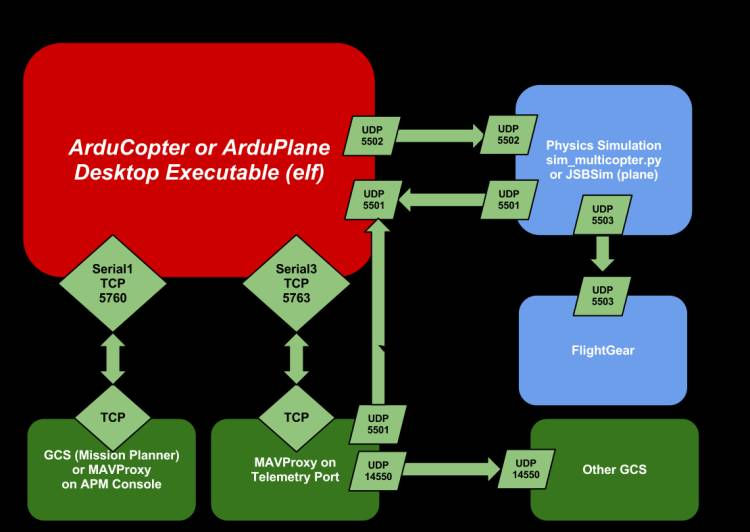
\includegraphics[width=0.65\textwidth]{Ardupilot_SITL.jpg}
    \caption{Ejemplo de puertos de comunicación de Ardupilot}
    \label{Ardupilot_SIL}
\end{figure}

\subsubsection{PymavLink}

De acuerdo con su documentación oficial \cite{MAVLink}, MAVLink es un protocolo para comunicación con drones y sus componentes; sigue un patrón de diseño híbrido de publicación-subscripción y comunicación punto-a-punto, en donde la trama de datos es enviada mediante el primer paradigma y los protocolos de configuración, como misiones y parámetros de vuelo, son enviados mediante el segundo.

En otras palabras, el uso del protocolo MAVLink es necesario para entablar comunicación con la simulación del controlador de vuelo provisto por Ardupilot, y de esta forma obtener los parámetros de vuelo de dron simulado así como el envío de comandos de vuelo.

Dicho lo anterior, MAVROS \cite{MAVROS} es un paquete de ROS que crea un nodo nativo capaz de entablar comunicación con un controlador de vuelo mediante MAVLink, por lo que es una alternativa bastante popular dentro de la comunidad, para la integración de software y proyectos relacionados con ROS y drones; sin embargo, a pesar de que el paquete se encuentre en constante desarrollo, la versión estable del mismo solo se está disponible para ROS 1, mientras que la implementación para ROS 2 todavía se encuentra en una etapa prematura de su desarrollo al tiempo de escritura de este trabajo, ofreciéndose en una versión alfa, la cual no cuenta con todas las funcionalidades ni con la estabilidad ofrecida por la implementación de ROS 1.


\section{Gazebo}

\subsection{Concepto}
Dentro del desarrollo de sistemas, es indispensable llevar a cabo un proceso de validación que permita evaluar el cumplimiento de los requerimientos funcionales del sistema desarrollado, tanto para software como para hardware. Hoy en día existen muchas herramientas que facilitan la ejecución de pruebas de validación para sistemas complejos; en este aspecto, el software de simulación corresponde a una gran alternativa pues permite realizar las pruebas de validación pertinentes bajo distintos paradigmas, en donde es necesario (o no) contar con un prototipo físico del sistema o un modelo matemático del mismo, lo anterior agiliza el desarrollo del sistema y probar algoritmos, diseños e incluso llevar a cabo el entrenamiento de algoritmos basados en inteligencia artificial; además, permite identificar errores y fallas en etapas tempranas del desarrollo del sistema, reduciendo costos y asegurando un mayor grado de calidad en el producto final.

De acuerdo con su sitio oficial \cite{gazebo_2014}, Gazebo es un software de simulación que ofrece la posibilidad de simular de forma precisa y eficiente, conjuntos de robots en ambientes complejos de interiores y exteriores. Además, ofrece un motor de físicas robusto, gráficos de alta calidad e interfaces gráficas y programáticas convenientes. Por último, al ser un proyecto desarrollado bajo el paradigma de open-source, cuenta con una comunidad bastante amplia que distribuye el conocimiento y se encarga de darle mantenimiento a este.

\subsection{Historia}
Creado por el Dr. Andrew Howard y su estudiante Nate Koeing, Gazebo comenzó su desarrollo en otoño de 2002 en la Universidad del Sur de California \cite{gazebo_2014}. El concepto de un simulador de alta fidelidad para robots, surgió a partir de la necesidad de simular este tipo de sistemas en ambientes bajo distintas condiciones. Gazebo fue nombrado de esta forma debido a que la estructura asociada a la palabra es un claro representante de un ambiente de exteriores; sin embargo, a pesar de que la mayoría de los usuarios de Gazebo lo utilizaban para simular ambientes de interiores, el nombre persistió hasta el día de hoy.

Con el paso de los años, Nate se encargó del desarrollo de Gazebo mientras terminaba su doctorado, y en 2009, John Hsu, un ingeniero en Willow garage, logró integrar ROS y el robot PR2 en Gazebo; desde entonces, Gazebo se convirtió en la herramienta de preferencia para llevar a cabo simulaciones de robots, por parte de la comunidad y usuarios de ROS.

Después, en la primavera de 2011, Willow Garage comenzó a financiar el desarrollo de Gazebo, y más tarde, en 2012, la Open Source Robotics Foundation (OSRF; que más tarde se convertiría en Open Robotics) surgiría como un organismo independiente a Willow Garage, continuando con el desarrollo de Gazebo. 

Hoy en día Open Robotics representa el equipo de desarrollo principal para Gazebo, en conjunto con la gran y diversa comunidad que ha acompañado al proyecto a lo largo de su desarrollo.

\subsection{¿Por qué Gazebo?}
A demás de las ventajas ya mencionadas, inherentes al uso de un simulador para la etapa de validación de un sistema, Gazebo cuenta con una serie de características que lo hacen único y por las cuales destaca.

\begin{itemize}
    \item \textbf{Proyecto de código abierto:} el código fuente de Gazebo está liberado al público, por lo que cualquier usuario experimentado puede entender su funcionamiento y contribuir a su desarrollo; además, al ser software libre, Gazebo puede ser utilizado por cualquier tipo de usuario prácticamente sin ningún tipo de restricción. 
    \item \textbf{Simulación de dinámicas:} es posible utilizar una serie de motores de físicas de código abierto, tales como ODE (Open Dynamics Engine), Simbody y DART (Dynamic Animation and Robotics Toolkit)
    \item \textbf{Gráficos avanzados en 3D:} Gazebo utiliza OGRE, un motor gráfico de código abierto que permite crear ambientes de simulación con gráficos realistas, incluyendo iluminación, sombras y texturas de alta calidad.
    \item \textbf{Sensores y ruido:} permite generar datos a partir de una amplia gama de sensores simulados, desde láseres, cámaras, sensores de movimiento, sensores de fuerza y torque, etc.
    \item \textbf{Plugins:} es posible desarrollar plugins personalizados para sensores, robots y el control de ambiente, con base en las necesidades del usuario. 
    \item \textbf{Modelos de robots:} Gazebo cuenta con un catálogo extenso de modelos de robots existentes en el mercado, que pueden ser utilizados por cualquier usuario; sin embargo, también existe la posibilidad de que el usuario cree su propio modelo de robot desde cero. 
    \item \textbf{Comunicación TCP/IP:} las simulaciones pueden ser ejecutadas desde servidores remotos y accedidas a partir de un protocolo de comunicación basado en el envío de mensajes por socket.
    \item \textbf{Simulación en la nube:} Gazebo puede ser ejecutado en una máquina virtual basada en la nube utilizando CloudSim y permite la interacción con la simulación a partir de su cliente web GzWeb.
    \item \textbf{Herramientas basadas en la línea de comandos:} Gazebo cuenta con un conjunto de herramientas para la línea de comandos que facilitan la interacción con la simulación en ejecución y así como su control.
\end{itemize}
